\documentclass[german, % Standardmäßig deutsche Eigenarten, englisch -> english
parskip=full, % Absätze durch Leerzeile trennen
bibliography=totoc, % Literatur im Inhaltsverzeichnis
%draft, % TODO: Entwurfsmodus -> entfernen für endgültige Version
]{scrartcl}
\usepackage{ifluatex} % zum Testen, ob LuaTeX verwendet wird
\ifluatex
\usepackage{fontspec} % Laden von Schriften
\setmainfont[Mapping=tex-text]{Linux Libertine O}  % Mapping ermöglicht die Verwendung z.B. von --
\setsansfont[Mapping=tex-text]{Linux Biolinum O}
\usepackage{polyglossia}  % Sprachpaket
\setdefaultlanguage[spelling=new,babelshorthands=true]{german}  % Neue Rechtschreibung und Abkürzungen
\else % kein LuaTeX
\usepackage[utf8]{inputenc} % Kodierung der Datei
\usepackage[T1]{fontenc} % Vollen Umfang der Schriftzeichen
\usepackage{lmodern}
\usepackage[ngerman]{babel} % Sprache auf Deutsch (neue Rechtschreibung)
%\usepackage{libertine} % Schriftart Linux Libertine/Biolinum verwenden
\fi

% Mathematik und Größen
\usepackage{amsmath}
\ifluatex
\usepackage{unicode-math}
\fi
\usepackage[locale=DE, % deutsche Eigenarten, englisch -> US
separate-uncertainty, % Unsicherheiten seperat
]{siunitx}
\usepackage{physics} % Erstellung von Gleichungen vereinfachen

% Bilder einbinden
\usepackage{graphicx}
\usepackage{float}
\usepackage{caption}
%\graphicspath{{bilder/}} % TODO: Pfad unter dem die Bilder gesucht werden

% Gestaltung
\usepackage{microtype}  % Mikrotypographie
\usepackage{booktabs}  %schönere Tabellen
\usepackage[toc]{multitoc}  %mehrspaltiges Inhaltsverzeichnis
\usepackage{csquotes} % Anführungszeichen mit \enquote
\usepackage{subcaption}  % Unterabbildungen a,b,c,…
\usepackage{enumitem}  % Listen anpassen
\setlist{itemsep=-10pt}
\usepackage{scrpage2}  % Manipulation des Seitenstils
% Kopf-/Fußzeilen
\pagestyle{scrheadings}
\clearscrheadings
\automark{section}
\ofoot{\pagemark}
\ihead{\headmark}
\setheadsepline{.5pt}

\usepackage[colorlinks=true]{hyperref}  % Links und weitere PDF-Features

\makeatletter 
\renewcommand\subsection{\@startsection 
   {subsection}{2}{0mm}%      % name, ebene, einzug 
   {0.5\baselineskip}%            % vor-abstand 
   {0.3\baselineskip}%            % nach-abstand 
   {\bfseries\sffamily\large}%           % layout 
   } 
\makeatother 

% TODO: Titel und Autor, … festlegen
\newcommand*{\titel}{Realstrukturanalyse}
\newcommand*{\autor}{Maximilian Obst, Thomas Adlmaier}
\newcommand*{\abk}{RA}
\newcommand*{\betreuer}{Dipl.-Phys. Rolf Schaarschuch}
\newcommand*{\messung}{11.11.2016}
\newcommand*{\ort}{Technische Universität Dresden, Institut für Strukturphysik}

\hypersetup{pdfauthor={\autor}, pdftitle={\titel}} % PDF-Metadaten

\titlehead{F-Praktikum \abk \hfill TU Dresden}
\subject{Versuchsprotokoll}
\title{\titel}
\author{\autor}
\date{\begin{tabular}{ll}
Protokoll: & \today\\
Messung: & \messung\\
Ort: & \ort\\
Betreuer: & \betreuer\end{tabular}}

%----------------
\begin{document}
\begin{titlepage}
\maketitle

\begin{figure}[hb] 
  \centering
     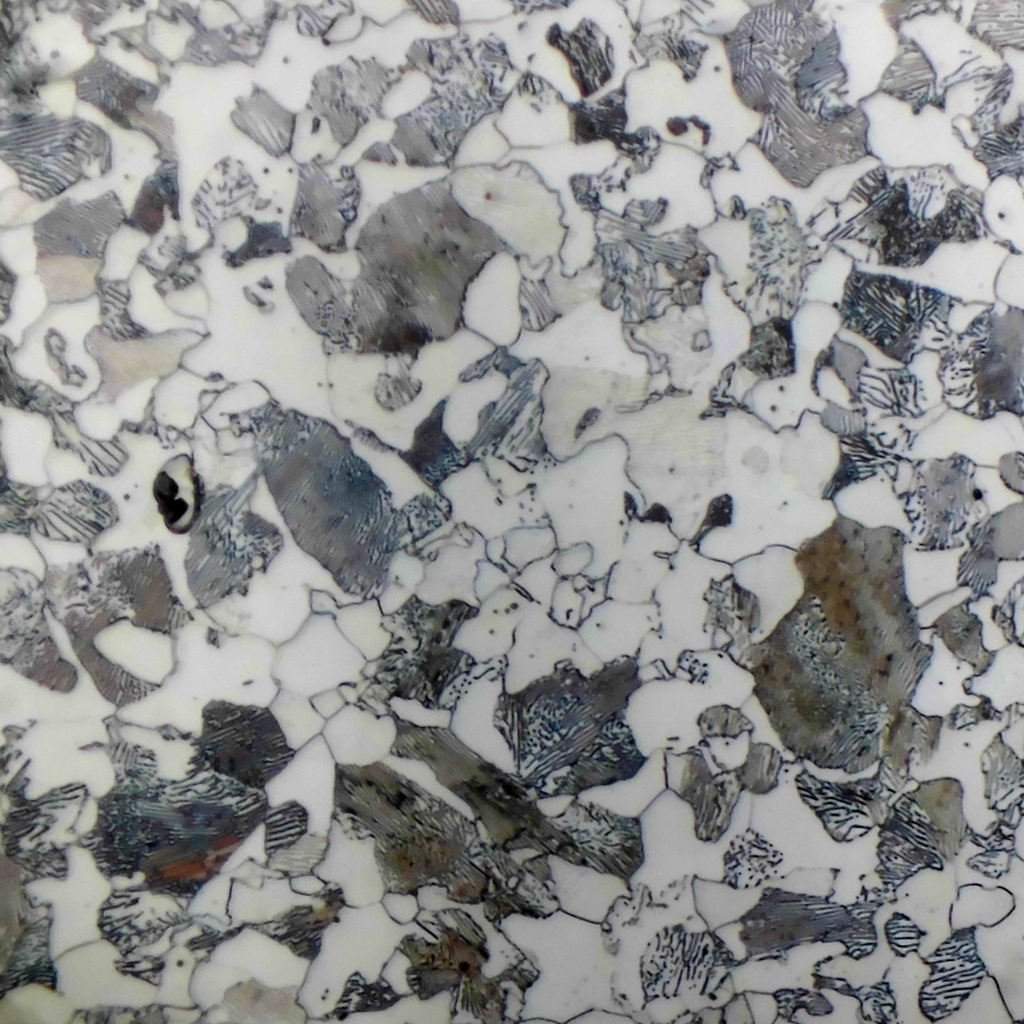
\includegraphics[width=0.7\textwidth]{RA_Bild}
  \caption{Stahl mit $0.45\,\%$ Kohlenstoffanteil	\cite{bild-ra}}
  \label{fig:tomographie}
\end{figure}
\end{titlepage}

\tableofcontents
\pagebreak

%------------------------
\section{Physikalische Grundlagen}

In der Realstrukturanalyse werden, anders als in der Idealstrukturanalyse, wo der perfekte Aufbau von Kristallgittern untersucht wird, Abweichungen von eben diesen Gittern betrachtet. In diesem Versuch werden die Oberflächen von einem Einkristall und zwei polykristallinen Systemen untersucht und damit ein Einblick in die Probenpräparation, metallographische Analyse und Bildverarbeitung geboten.

\subsection{Gitterdefekte}

Gitterdefekte beschreiben Abweichungen vom perfekten Kristall. Sie werden in folgende Gruppen unterschieden: \cite{gitterfehler}

\subsubsection{Nulldimensionale Gitterdefekte}

Auch Punktdefekte genannt. Diese Defekte beschreiben Abweichungen an einzelnen Atompositionen:
\begin{itemize}
\item \textbf{Leerstellen:} Fehlende Gitteratome
\item \textbf{Zwischengitteratome:} Zusätzliche Atome zwischen den eigentlichen Gitteratomen
\item \textbf{Substitutionsatome:} Atome eines anderen Elementes, die anstelle der eigentlichen Gitterelementes im Gitter eingebunden sind
\end{itemize}

\subsubsection{Eindimensionale Gitterdefekte}

Auch Linienfehler genannt. Hier werden Abweichungen beschrieben, die eine ganze Reihe von Atomen betreffen:
\begin{itemize}
\item \textbf{Stufenversetzung:} Eingeschobene Halbebenen im Kristallgitter, die zu einer Verschiebung führen
\item \textbf{Schraubenversetzung:} Gegeneinander senkrecht halb-verschobene Ebenen im Kristall (ein Teil verschoben, der andere nicht)
\end{itemize}

\subsubsection{Zweidimensionale Gitterdefekte}

Auch Flächenfehler genannt. Diese beschreiben Abweichungen, die in der Fläche beobachtet werden können:
\begin{itemize}
\item \textbf{Korngrenzen:} Grenzflächen zweier gegeneinander verdrehter Einkristalle
\item \textbf{Zwillingsgrenzen:} Grenzflächen beider Teile eines Kristallzwillings
\item \textbf{Stapelfehler:} Verschiebung der aufgestapelten Ebenen, sodass das Gitter falsch aufgebaut wird
\item \textbf{Phasengrenzen:} Grenzflächen zweier Phasen eines polykristallinen Systems
\end{itemize}

\subsubsection{Dreidimensionale Gitterdefekte}

Auch Volumenfehler oder Inklusionen genannt. Dies sind Abweichungen, die durch vollständige Fremdphasen im Kristallgitter entstehen:
\begin{itemize}
\item \textbf{Poren:} Hohlräume im Kristall, die mit Gas oder Flüssigkeit gefüllt sind
\item \textbf{Einschlüsse:} Im Kristall enthaltene andere feste Materialien
\item \textbf{Ausscheidungen:} Einschlüsse, die aus dem Kristall selbst gebildet werden
\end{itemize}

\subsection{Silicium}

Silicium ist ein Halbmetall in der vierten Hauptgruppe des Periodensystems der Elemente. Es wird in elementarer Form hauptsächlich als Halbleiter genutzt. Der Silicium-Kristall weist eine Diamantstruktur auf.

Die Elementarzelle der Diamantstruktur besteht aus einer kfz-Strukur mit einer Basis {(0,0,0),(1/4,1/4,1/4)}. Findet eine Versetzung in der Struktur statt, so bilden sich je nach Richtung des Kristalls unterschiedliche Muster beim Ätzen aus: Weist der Kristall eine (1,0,0)-Richtung auf, so bilden sich Quadrate. Hat der Kristall eine (1,1,0)-Richtung, können Linsen gesehen werden, bei einer (1,1,1)-Richtung formen sich gleichseitige Dreiecke.

\subsection{Messing}

Messing ist eine Legierung aus Kupfer und Zink. Je nach der größe der Anteile der beiden Elemente entstehen drei unterschiedliche Phasen: $\alpha$-Messing, $\beta$-Messing und $\gamma$-Messing. Dabei wird industriell hauptsächlich $\alpha$- und $\beta$-Messing hergestellt und benutzt.

$\alpha$-Messing hat einen Kupfergehalt von über $62.5\,\%$ und weist eine kfz-Struktur auf. Es besitzt eine gute Formbarkeit bei Raumtermperatur und eine hohe Korrosionsbeständigkeit. Eine Anwendungsmöglichkeit ist die Verwendung als Schmuck oder Münzmaterial, auch in der Uhrenherstellung findet es Anwendung. \cite{messing}

$\beta$-Messing hat einen Kupfergehalt zwischen $54$ und $62.5\,\%$ und weist eine krz-Struktur auf. Es besitzt eine gute Formbarkeit im warmen Zustand. Durch Zugabe von $0.5$ bis $3.5\,\%$ Blei erreicht $\beta$-Messing zusätzlich eine hohe Zerspanbarkeit und wird daher gerne für industrielle Bauteile verwendet.

\begin{figure}[hb] 
  \centering
     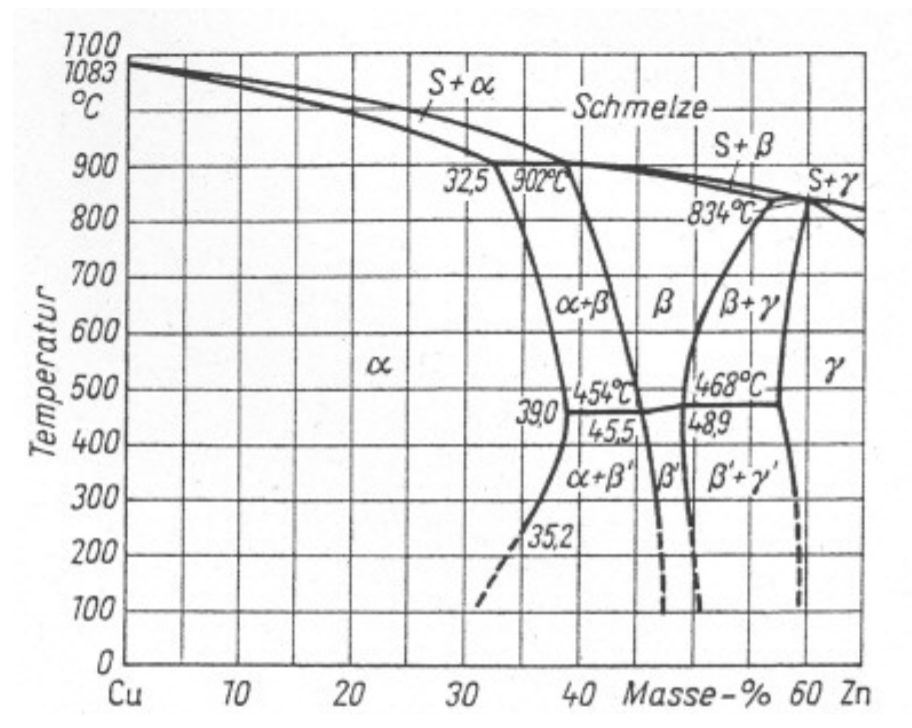
\includegraphics[width=0.8\textwidth]{Messing_Phase}
  \caption{Phasendiagramm von Messing}
  \label{fig:phasemessing}
\end{figure}

\subsection{Stahl}

Stahl ist eine Legierung aus Eisen und Kohlenstoff. In dieser Legierung können, in der Reihenfolge aufsteigendem Kohlenstoffgehalts, vier Phasen beobachtet werden: $\alpha$-Eisen, $\delta$-Eisen, $\gamma$-Eisen und Fe\textsubscript{3}C. Dabei hat Zementit mit einem Kohlenstoff-Masseanteil von $6.67\,\%$ die maximale Menge an Kohlenstoff, die Eisen binden kann, gebunden. 

$\alpha$-Eisen, auch Ferrit genannt, hat einen maximalen Kohlenstoffgehalt von $0.02\,\%$. Die Eisenatome weisen eine krz-Struktur auf, bei der die Kohlenstoffatome zwischengelagert sind. Ferrit ist sehr weich und formbar, weist dabei eine geringe Wärmeausdehnung auf und ist ferromagnetisch. Allerings ist Ferrit nicht sehr wärmebeständig. \cite{ferrit}
$\delta$-Eisen wird auch $\delta$-Ferrit genannt und weist die selbe Struktur wie $\alpha$-Eisen auf. Der Kohlenstoffgehalt liegt bei höchstens $0.1\,\%$. 
$\gamma$-Eisen hat auch die Bezeichnung Austenit. Hier bilden die Eisen-Atome eine kfz-Struktur, die Kohlenstoff-Atome sind wieder zwischengelagert. Der Kohlenstoffgehalt liegt mit bis zu $2.06\,\%$ deutlich höher als bei den Ferriten. Austenit ist sehr zäh und bricht damit seltener als Ferrit. Außerdem leitet Austenit Wärme schlecht, ist paramagnetisch und bei hohen Temperaturen sehr fest. Austenit zeigt dabei aber auch eine hohe Wärmeausdehnung und eine niedrige Festigkeit bei niedrigen Temperaturen. \cite{austenit}
Fe\textsubscript{3}C wird Zementit genannt und stellt mit $6.67\,\%$ Kohlenstoffanteil die Eisen-Kohlenstoff-Verbindung da, die die höchstmögliche Menge an Kohlenstoff bindet. Die gebildete, komplizierte Struktur besteht aus Tetraedern, in denen ein Kohlenstoff-Atom von 4 Eisen-Atomen umgeben wird. Zementit ist in nahezu allen Stählen enthalten. Dabei werden beim Stahl bestimmte Anteile von Zementit unterschieden: Perlit hat $88\,\%$ Ferrit und $12\,\%$ Zementit. Ledeburit I hat einen Austenit-Anteil von $52.4\,\%$ und einen Zementit-Anteil von $47.6\,\%$. Ledburit II schließlich hat einen Perlit-Anteil von $51.4\,\%$ und einen Zementit-Anteil von $48.6\,\%$.

\begin{figure}[hb] 
  \centering
     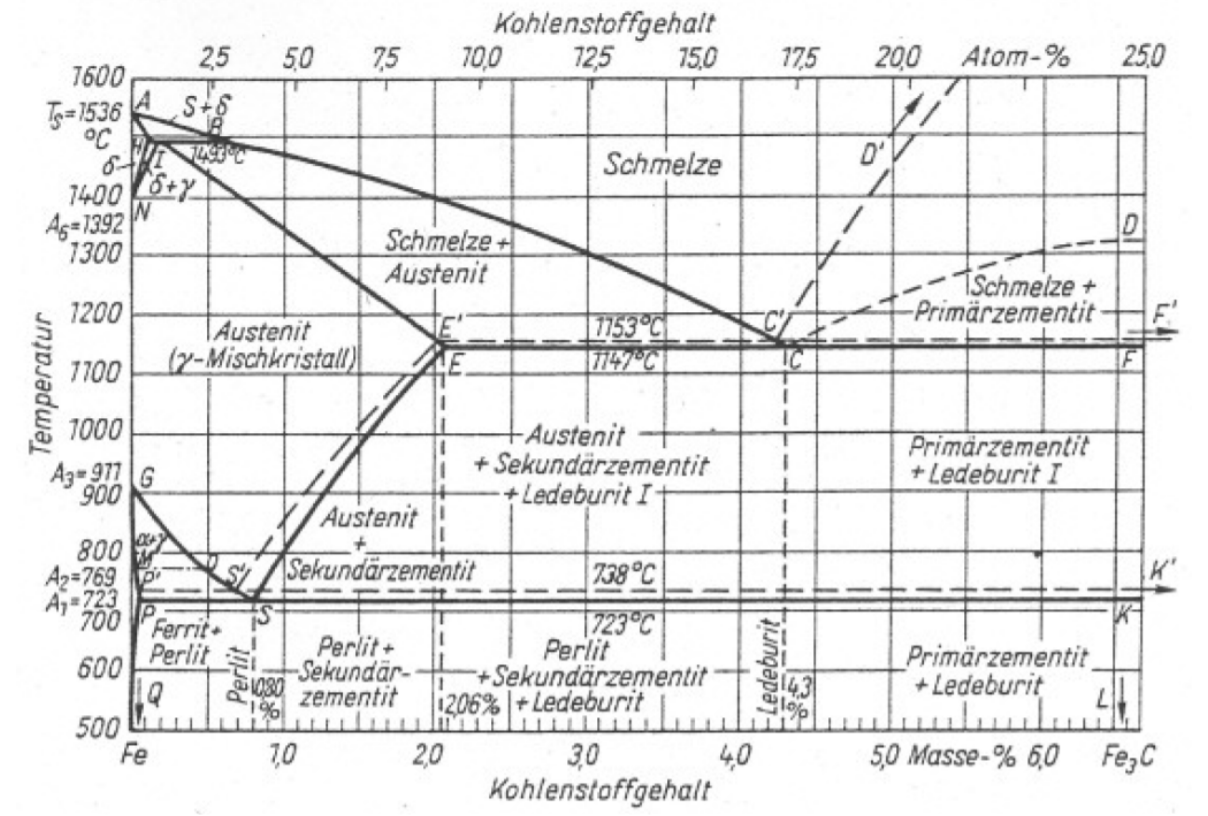
\includegraphics[width=0.8\textwidth]{Stahl_Phase}
  \caption{Phasendiagramm von Stahl}
  \label{fig:phasestahl}
\end{figure}

\section{Durchführung}

In diesem Versuch soll ein Silicium-Einkristall auf Stufenversetzungen sowie Messing und Stahl auf ihre Atombestandteile in Gewichtsprozent untersucht werden. Für die Untersuchung werden die Materialien geschliffen und angeätzt, um anschließend mit Auflicht-Mikroskopen betrachtet zu werden.

\subsection{Silicium}

Um die Versetzungsstruktur des Silicium-Einkristalls zu beobachten, muss der Kristall an geeigneten kristallographischen Flächen geläppt und chemisch angeätzt werden. Für jedes Ätzen muss der Kristall in die entsprechende Säure gehalten, danach in Wasser und destilliertem Wasser gereinigt werden um schließlich in Ethanol 3 Minuten in einem Ultraschallbad weiter gereinigt zu werden. Als letztes wird der Kristall aus dem Ethanol entnommen und so lange mit einem Heißluft-Föhn beblasen, bis er trocken ist. 
\begin{itemize}
\item[1.] Als erstes muss der Kristall geläppt werden. Dafür wird der Kristall an den zu bearbeitenden Flächen über eine mit Läpppulver F40 und Wasser versehene Glasplatte gerieben werden, bis die Flächen mattgrau sind.
\item[2.] Dann wird der Kristall das erste Mal geätzt. Hier wird eine Säure aus gleichen Anteilen Fluss- und Salpetersäure verwendet und der Kristall $25\,s$ in dieser geschwenkt
\item[3.] Nun wird der Kristall das erste Mal unter dem Mikroskop betrachtet. Dabei wird der Kristall zuerst fokussiert und dann ein Bild gemacht
\item[4.] Als nächstes wird der Kristall das zweite Mal geätzt. Jetzt wird eine Säure aus einem Bestandteil Fluss- und fünf Bestandteilen Salpetersäure genutzt und der Kristall $30\,s$ in dieser geschwenkt
\item[5.] Es folgt die zweite Betrachtung des Kristalls unter dem Mikroskops. Nun sollen die ersten Versetzungen gefunden und fokussiert werden. Die Versetzungen sind dabei anhand ihrer klaren geometrischen Struktur zu erkennen. Von den gefunden Versetzungen wird ein Bild gemacht
\item[6.] Anschließend folgt die dritte Verätzung. Es wird eine Säure aus gleichen Bestandteilen Stammlösung (\(\SI{50}{\gram}\) CrO\textsubscript{3} auf \(\SI{100}{\milli\liter}\) Wasser) und Flusssäure verwendet und der Kristall $15\,s$ in dieser geschwenkt
\item[7.] Danach wird der Kristall ein drittes Mal unter dem Mikroskop betrachtet. Dabei werden wieder die Versetzungsstellen betrachtet und fotografiert
\end{itemize}

\subsection{Messing und Stahl}

Um bei Messing und Stahl die Gefügestruktur zu untersuchen, müssen geeignete metallografische Flächen geschliffen, poliert und geätzt werden. Das Schleifen und Polieren ist dabei für Messing und Stahl identisch. 

\begin{itemize}
\item[1.] Die zu betrachteten Flächen werden mit einem SiC-Papier unterschiedlicher Körnung geschliffen. Dabei wird die Größe der Schleifkörner immer weiter verkleinert: Erst wird die Körnung 500 verwendet, dann 1000 und schließlich 2000
\item[2.] Danach werden die Flächen mit einer \(\SI{3}{\micro\meter}\) Diamantsuspension poliert, bis sie metallisch glänzen
\end{itemize}

Nun müssen die Legierungen geätzt werden, um anschließend im Mikroskop betrachtet zu werden. Nach jedem Ätzen müssen die Legierungen in Ethanol gereinigt werden um anschließend mit einem Heißluft-Föhn getrocknet zu werden. Diese Schritte werden wiederholt, bis die Bestandteile gut gesehen werden können:

Messing in einem Ätzmittel aus \(\SI{100}{\milli\liter}\) Wasser, \(\SI{30}{\milli\liter}\) HCL und $5\,g$ FeCl\textsubscript{3} $25\,s$ geschwenkt, anschließend im Mikroskop fokussiert und ein Foto geschossen.

Stahl wird in einer $3\,\%$igen alkoholischen Salpetersäure \(\SI{10}{\second}\) geätzt und anschließend ebenfalls im Mikroskop fokussiert und ein Foto geschossen.

\section{Analyse}

\subsection{Silicium}

\begin{figure}[ht] 
  \centering
     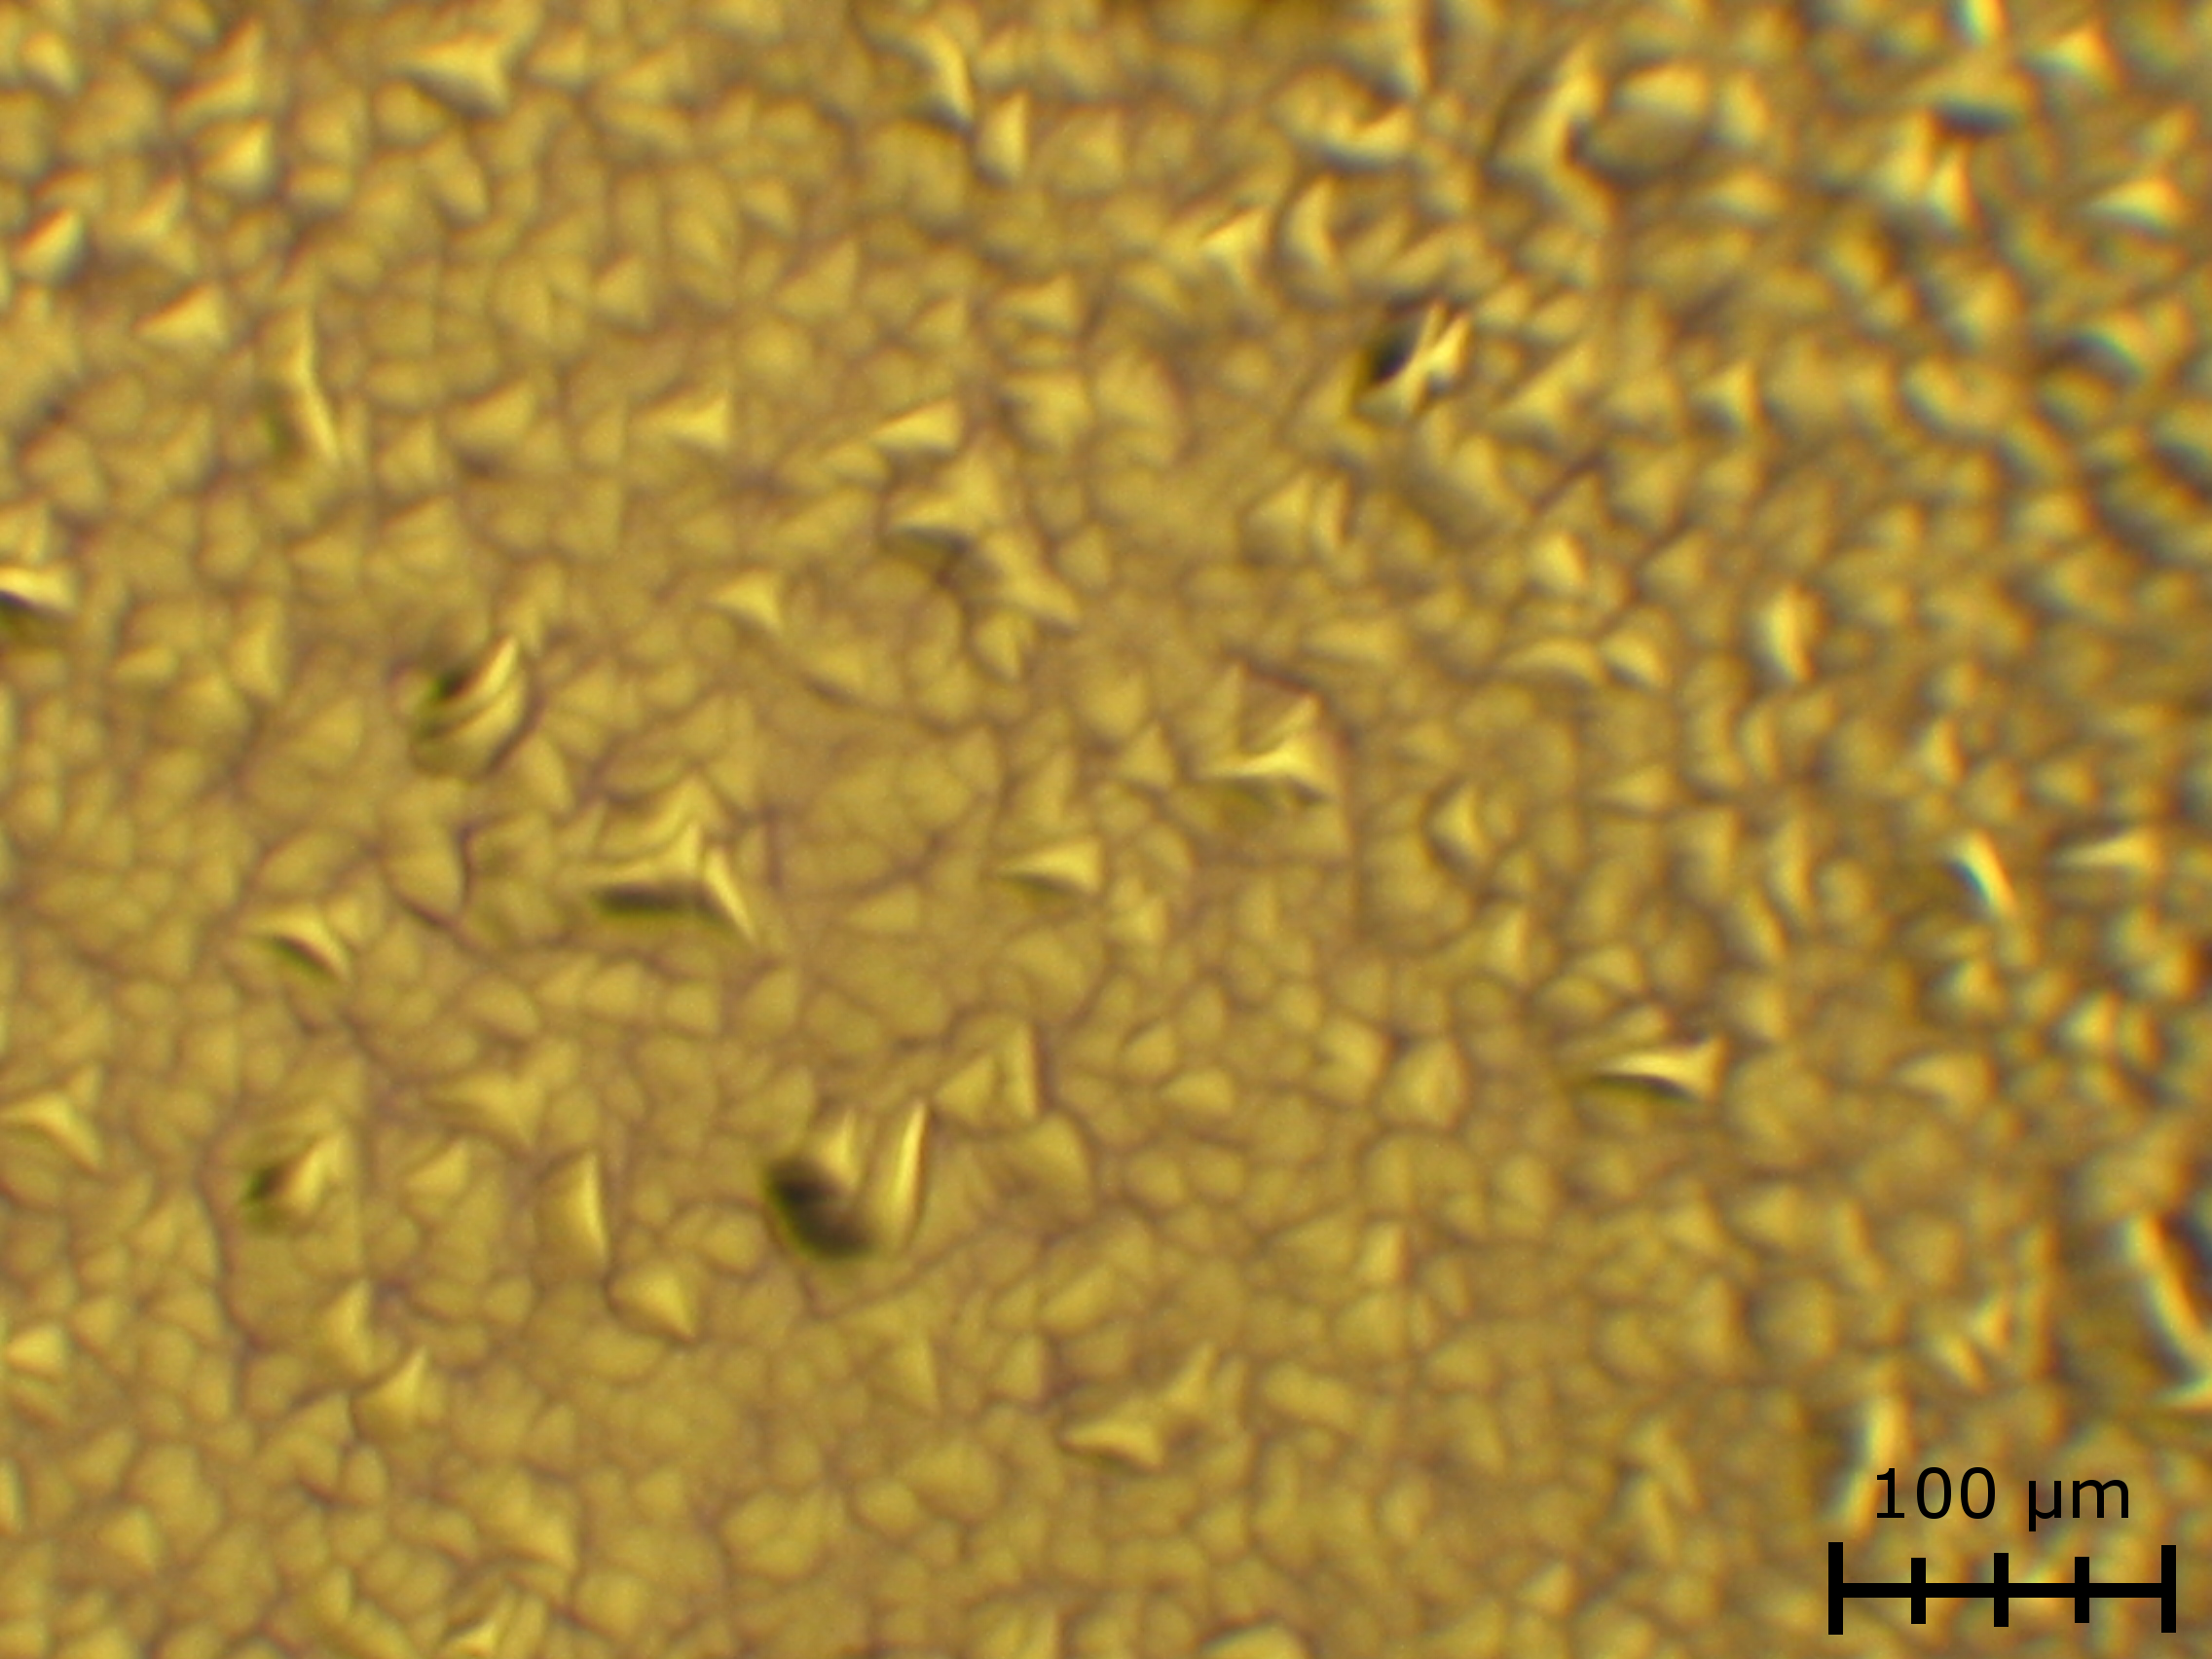
\includegraphics[width=0.8\textwidth]{Silicium_1_12}
  \caption{Silicium nach 1 Arbeitsschritt unter 12.5-facher Vergrößerung}
  \label{fig:sil112}
\end{figure}

Nach dem ersten Arbeitsschritt zeigt sich im Bild \ref{fig:sil112} unter 12.5-facher Vergrößerung eine erste grobe Struktur der Oberfläche. Dabei sind die hellen Flächen leichte Erhebungen, während die dunklen Linien Senken zwischen den Erhebungen sind. Zudem sind Schäden in der Oberflächenstrkutr zu erkennen, die wie Kerben aussehen.

\begin{figure}[ht] 
  \centering
     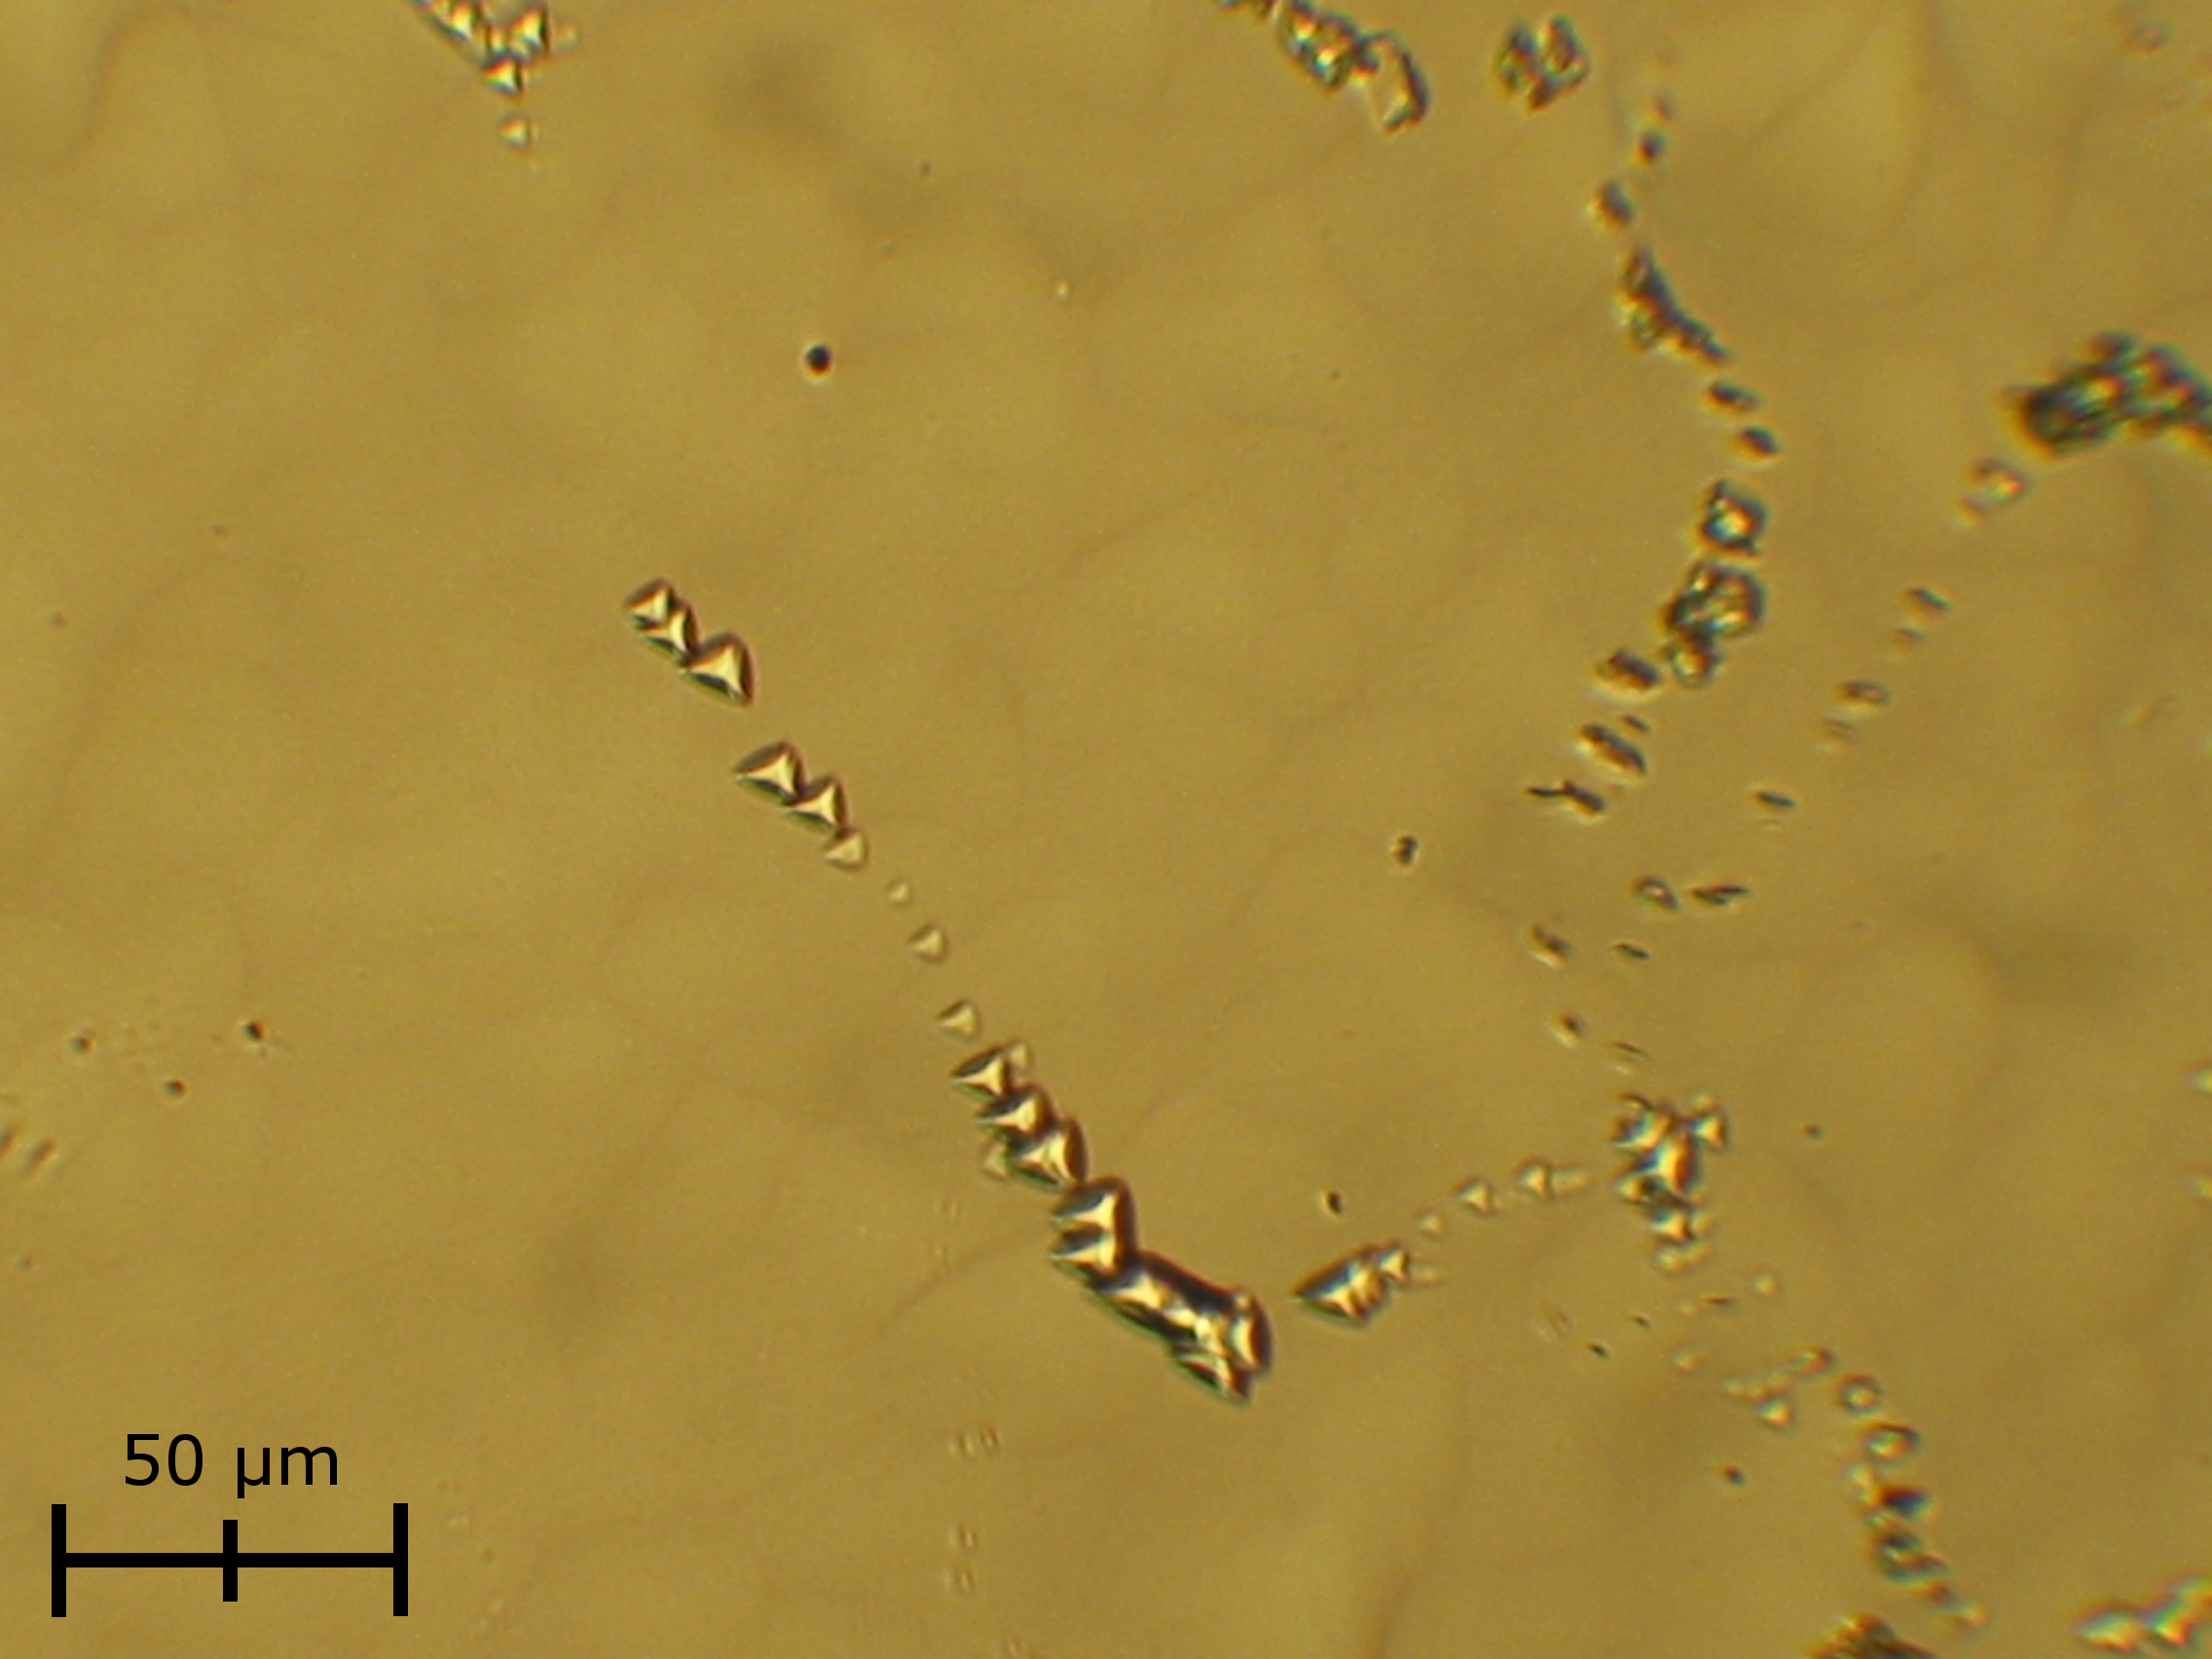
\includegraphics[width=0.8\textwidth]{Silicium_2_25}
  \caption{Silicium nach 2 Arbeitsschritten unter 25-facher Vergrößerung}
  \label{fig:sil225}
\end{figure}

Nach dem zweiten Arbeitsschritt zeigt sich unter 25-facher Vergrößerung in Bild \ref{fig:sil225} eine klare Veränderung: Die Erhebungen und Senken sind kaum noch zu sehen, dafür erste Feinstrukturen der Oberfläche. In der oberen rechten Ecke des Bildes sind dunkle, unförmige Kerben zu erkennen, deren Ursache nur über das Bild nicht klar erklärbar ist. In der Mitte des Bildes können hellere Dreiecke erkannt werden, die im unteren Teil des Bildes inneinanderlaufen. 

\begin{figure}[ht] 
  \centering
     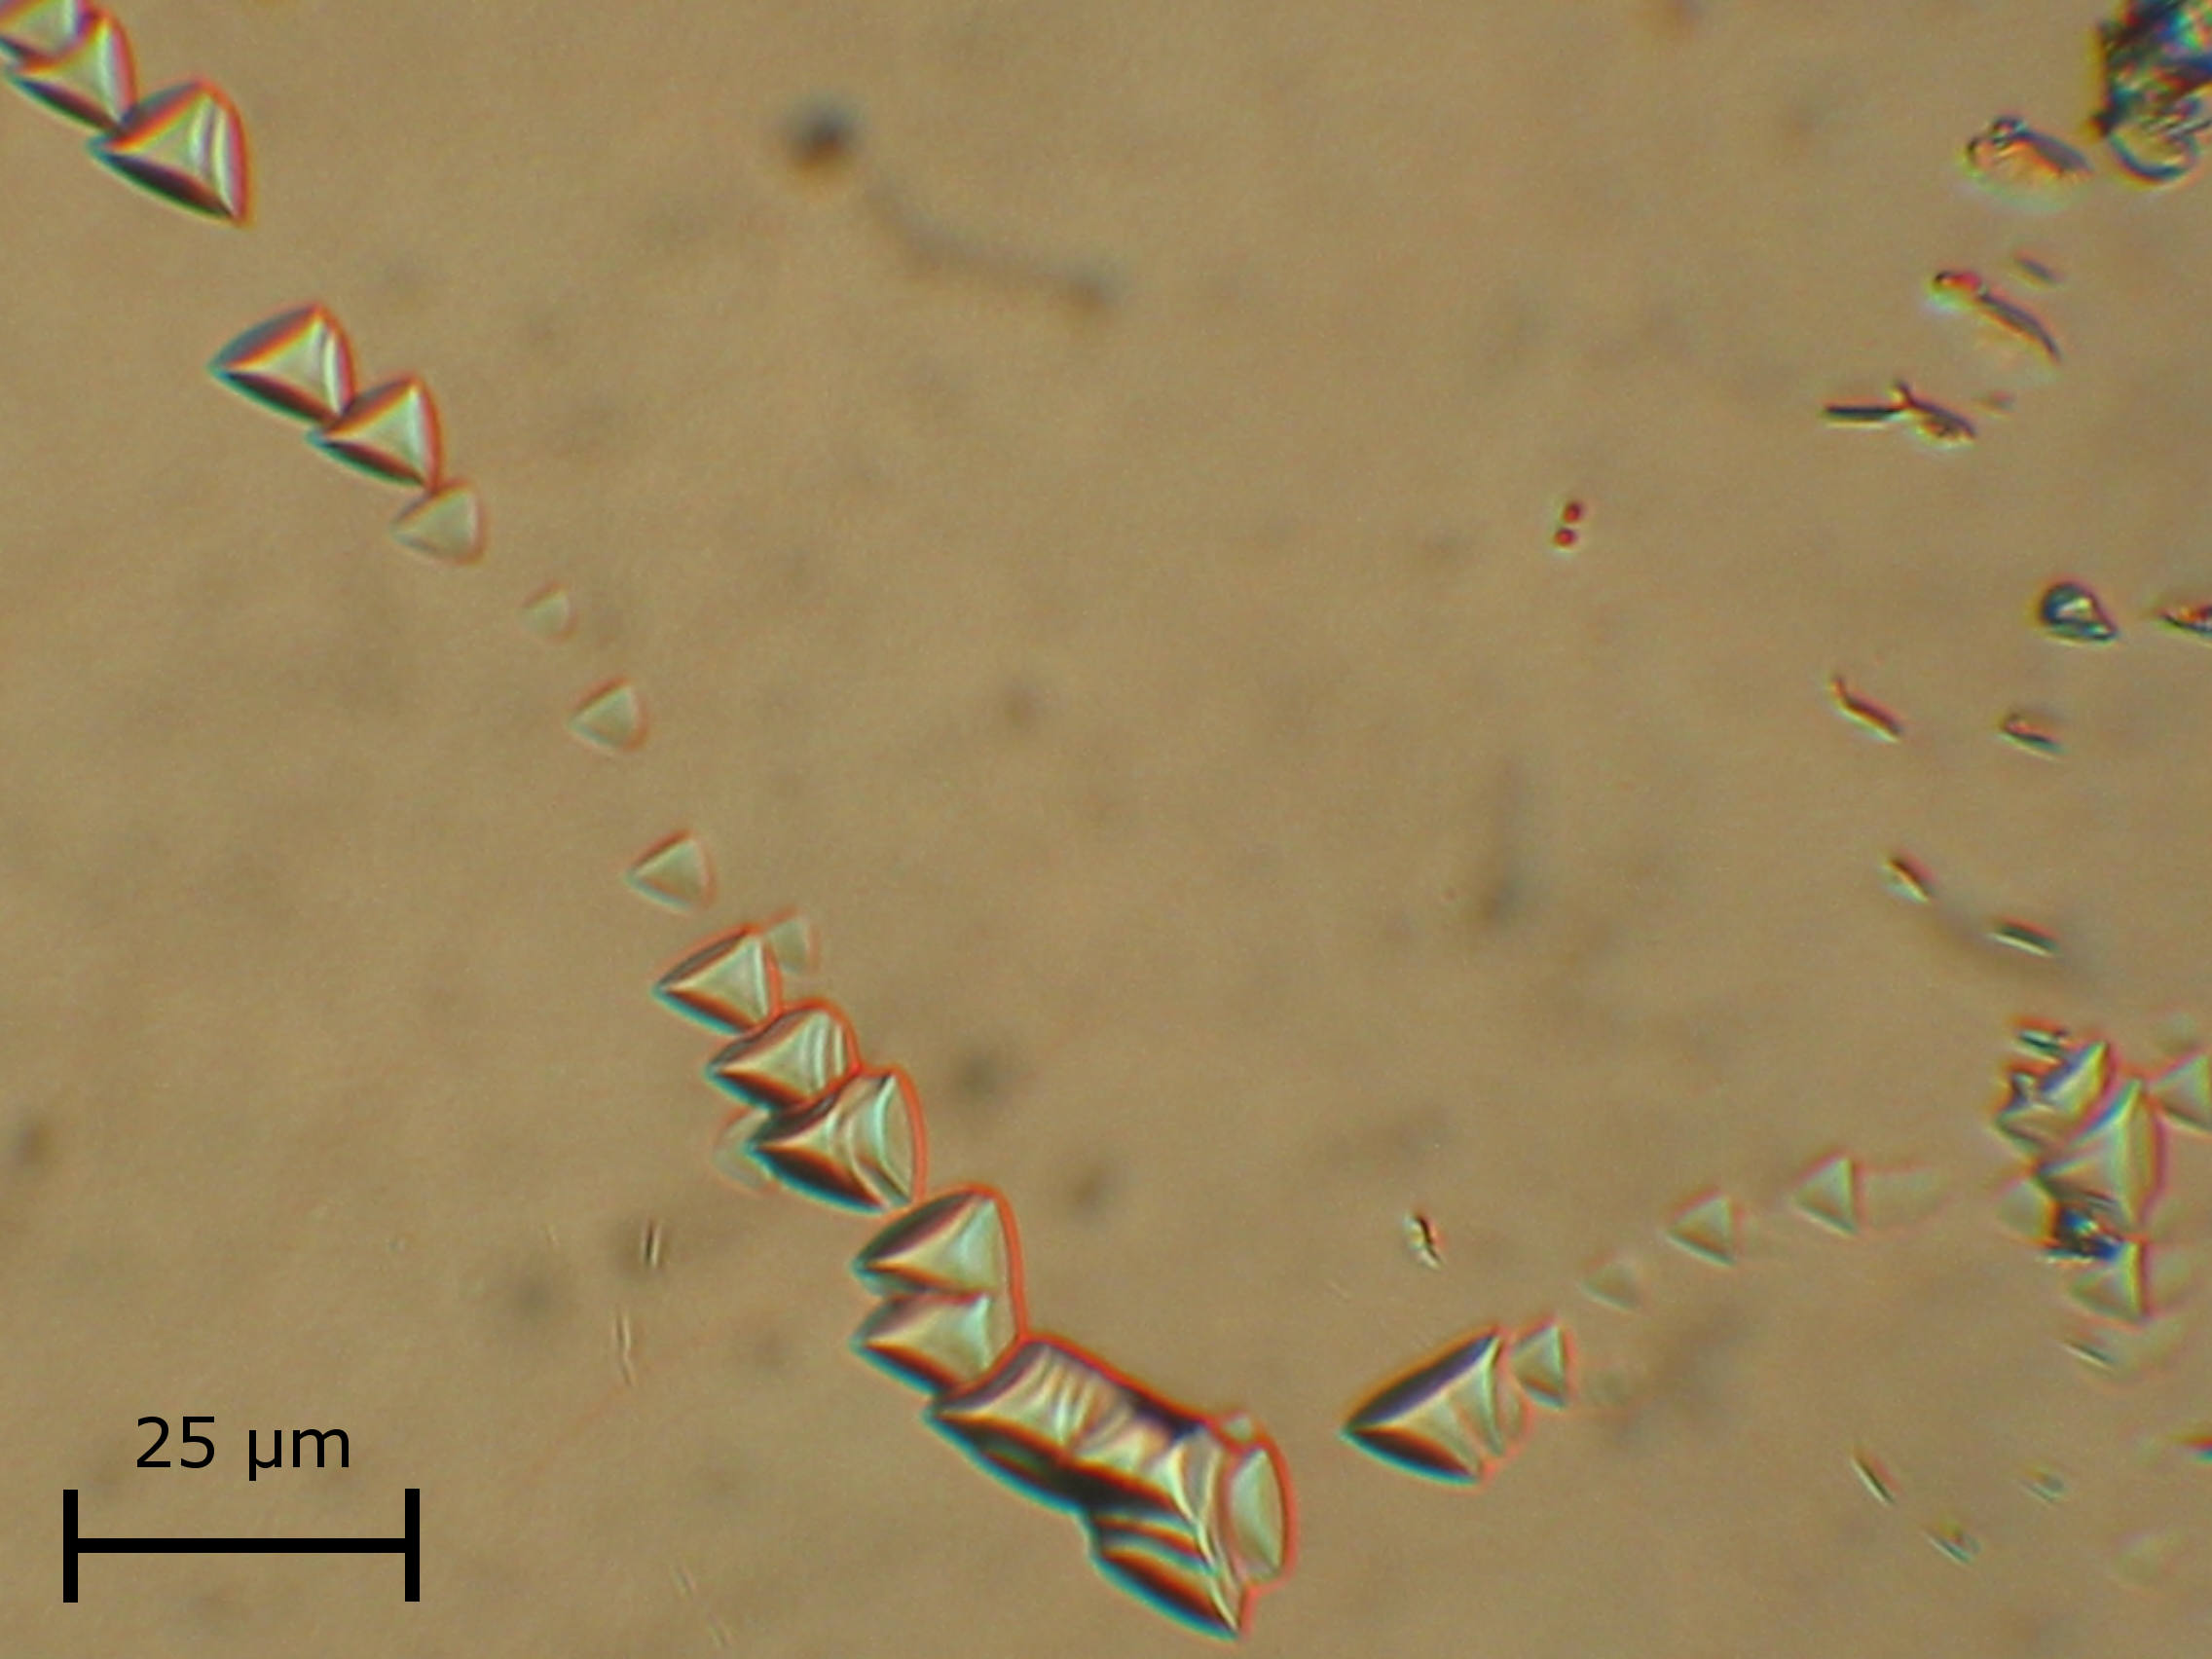
\includegraphics[width=0.8\textwidth]{Silicium_2_50}
  \caption{Silicium nach 2 Arbeitsschritten unter 50-facher Vergrößerung}
  \label{fig:sil250}
\end{figure}

Mit einer stärkeren Vergrößerung in Bild \ref{fig:sil250} lässt sich erkennen, dass tatsächlich alle hellere Flecken aus gleichseitigen Dreiecken bestehen. Diese entstehen durch Versetzungen im Kristall. Dass die Form ein gleichseitiges Dreieck ist, lässt darauf schließen, dass der Silicium-Einkristall in (1,1,1)-Richtung gezogen wurde.

\begin{figure}[ht] 
  \centering
     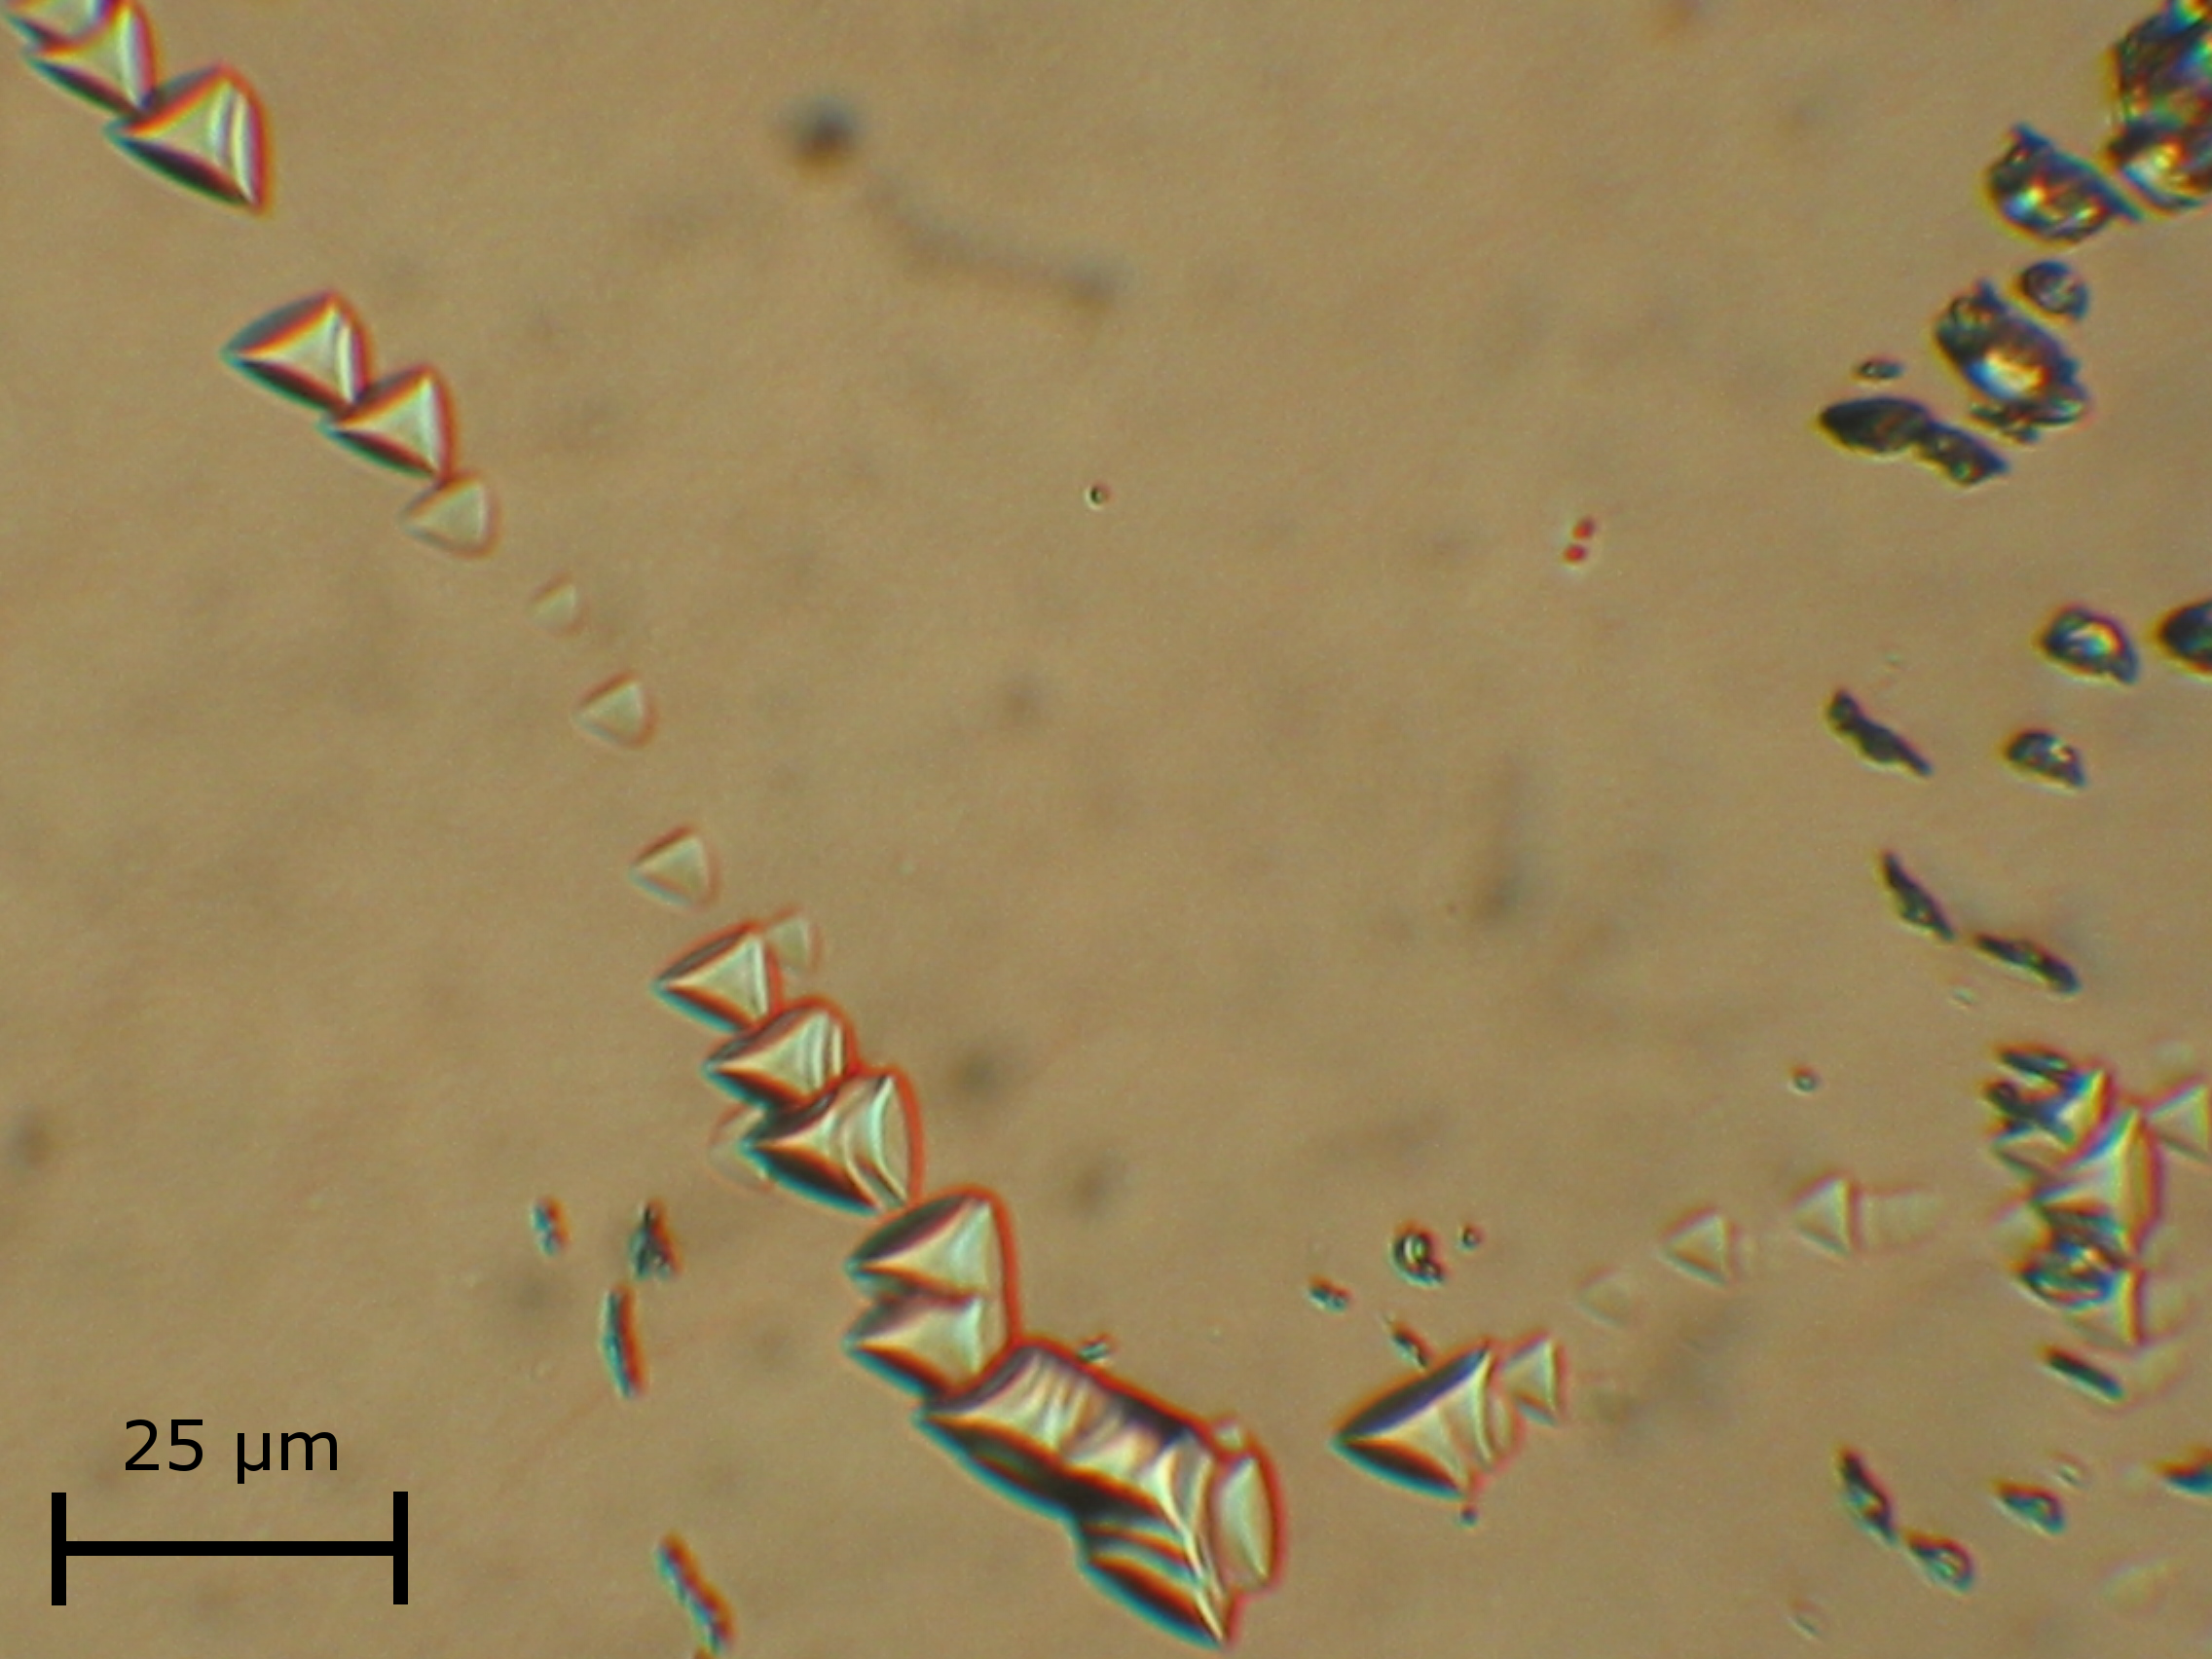
\includegraphics[width=0.8\textwidth]{Silicium_3_50}
  \caption{Silicium nach 3 Arbeitsschritten unter 50-facher Vergrößerung}
  \label{fig:sil350}
\end{figure}

Nach dem dritten und letzten Arbeitsschritt verändert sich das Aussehen nicht mehr grundlegend, wie in Bild \ref{fig:sil350} gesehen werden kann. Auffällig ist vor allem die Vergrößerung der unförmigen Kerben. 

\begin{figure}[ht] 
  \centering
     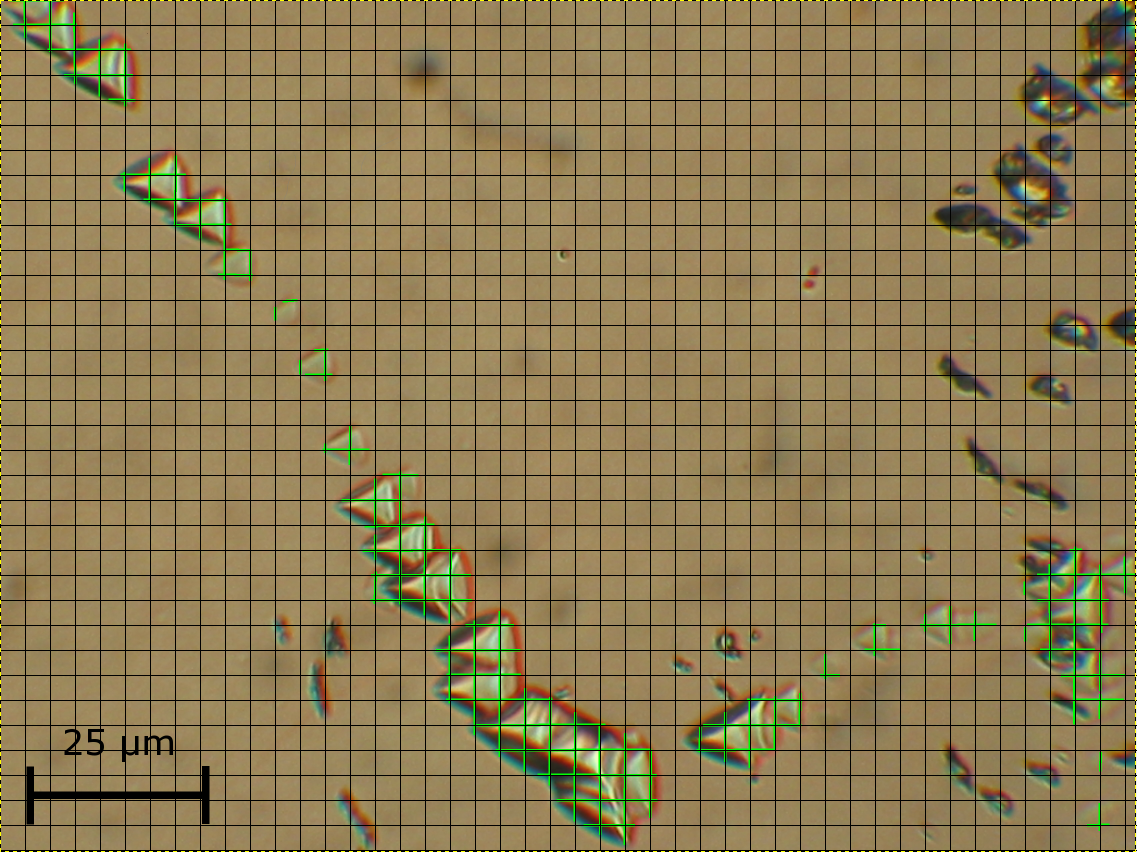
\includegraphics[width=0.8\textwidth]{Silicium_3_50_mal2}
  \caption{Linearanalyse von Bild \ref{fig:sil350}}
  \label{fig:linana}
\end{figure}

In diesem Bild wird auch die Analyse durchgeführt. Ein Ausmessen der Dreiecke mit einem Bildverarbeitungsprogramm ergibt, dass die Seitenlängen der Dreiecke zwischen \(\SI{4}{\micro\meter}\) und \(\SI{14}{\micro\meter}\) schwankt. Mit der Durchführung einer Linearanalyse gelangt man zu folgendem Schluss:
\begin{align*}
L_L = 0.0714
\end{align*}
Dies gilt dabei nur für das betrachtete Bild und nicht für den gesamten Kristall! Bei der Durchführung konnte beobachtetet werden, dass die meisten Stellen der einen betrachteten Oberflächen keinerlei Versetzungen aufweisen, die andere betrachtete Oberfläche besaß keine einzige Versetzung. Daher liegt der wahre Wert für L\textsubscript{L} viel geringer. In Bild \ref{fig:linana} kann die angewandte Methode der Linearanalyse nachvollzogen werden.

\begin{figure}[ht] 
  \centering
     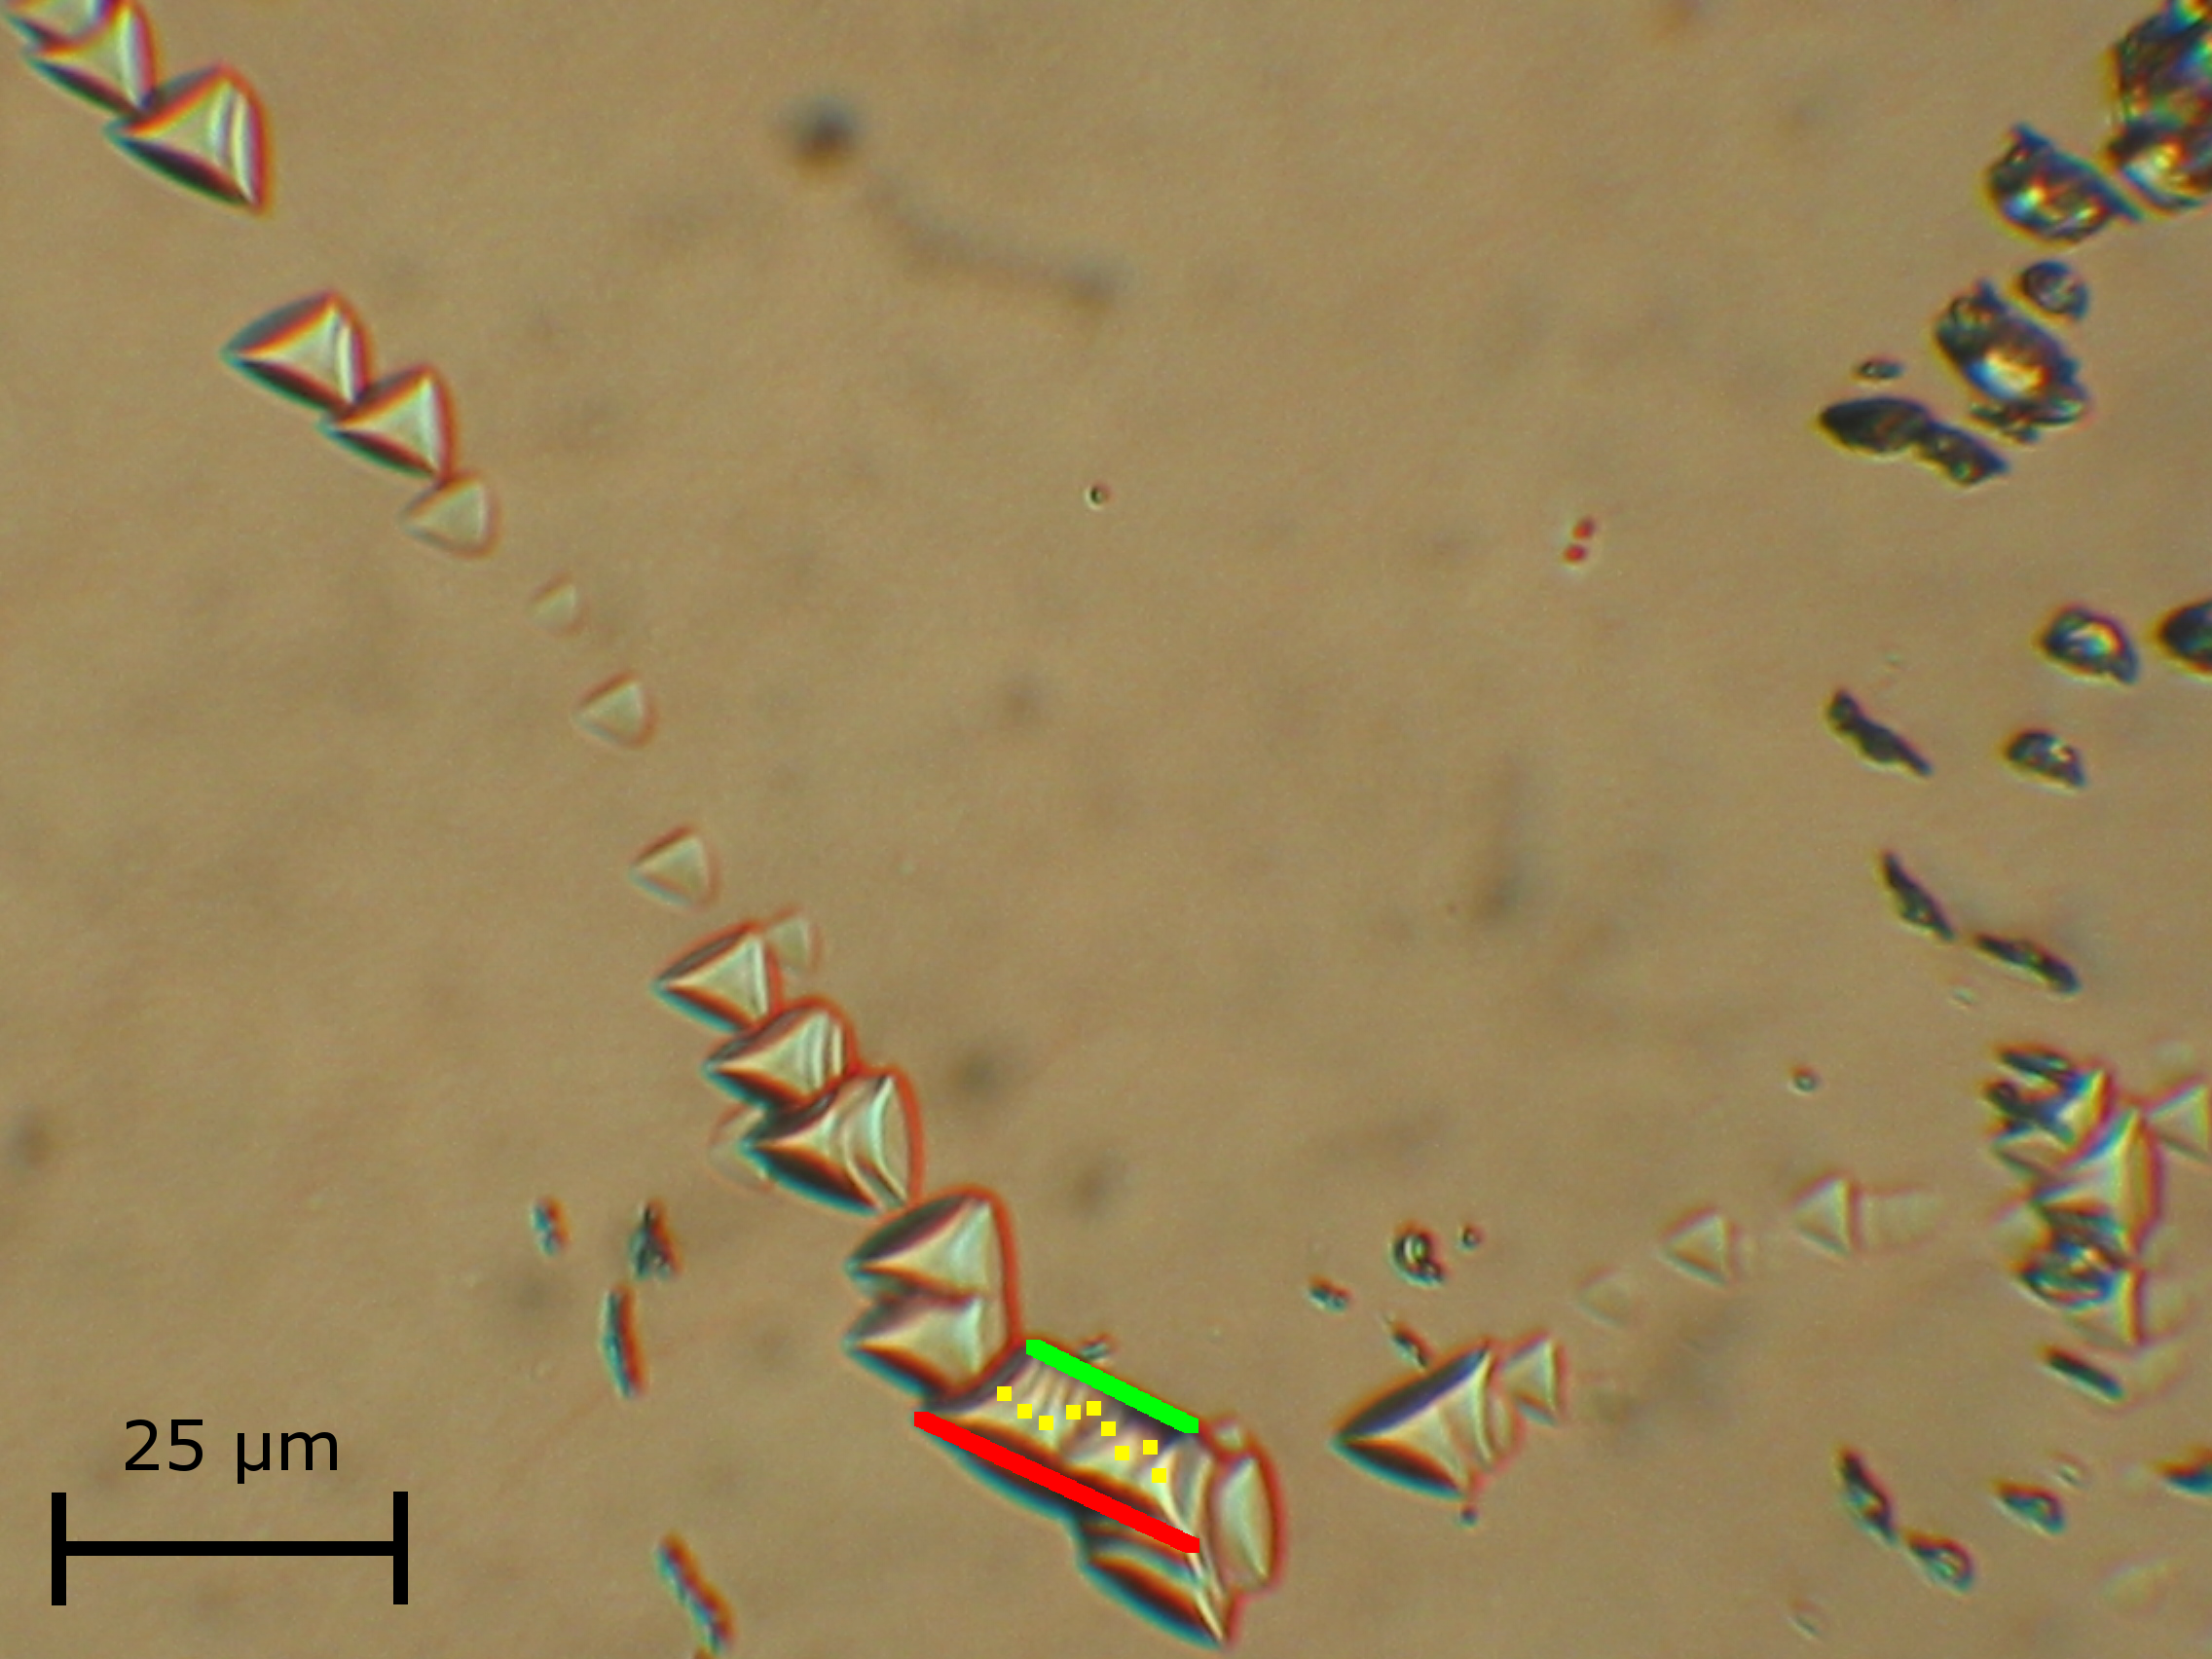
\includegraphics[width=0.8\textwidth]{Silicium_3_50_mal_verkippung}
  \caption{Bestimmung des Verkippungswinkels}
  \label{fig:verkippung}
\end{figure}

Zur Bestimmung des Verkippungswinkels zwischen den Subkörnern wird die unten im Bild erkennbare, kurze, gerade Linie von Versetzungen oben und unten vermessen, wie in Bild \ref{fig:verkippung} zu sehen ist. Zusätzlich wird die Zahl der an der Linie beteiligten Versetzungen bestimmt. Dann wird die Weglänge je Versetzung mit der Formel \ref{for:lversetzung} bestimmt.
\begin{align}
D_{Versetzung} = \frac{l_{oben} + l_{unten}}{2} \frac{1}{N_{Versetzungen}} \label{for:lversetzung}
\end{align}
Das Ergebnis in Mikrometern lautet wie folgt:
\begin{align*}
D_{Versetzung} = \SI[separate-uncertainty = true]{1.9(4)}{\micro\meter}
\end{align*}
Der Burgersvektor $b_{Silizium}$ von Silicium wird mithilfe der Formel \ref{for:burgers} berechnet. Dabei wird genutzt, dass der Kristall, wie oben beschrieben, in (1,1,1)-Richtung gezogen wurde und Silizium eine Gitterkonstant von $a = \SI{5.430}{\angstrom}$ \cite[S.24]{kittel}. Somit gilt $h = k = l = 1$. Mit diesen beiden Werten und der Formel \ref{for:verkippung} kann der Verkippungswinkel bestimmt werden \cite[S.661]{kittel}.
\begin{align}
b_{Silizium} = \frac{a_{Silizium}}{2}\sqrt{h^2+k^2+l^2} \label{for:burgers}
\end{align}
\begin{align}
\Theta_{Verkippung} = \frac{b_{Silizium}}{D_{Versetzung}} \label{for:verkippung}
\end{align}
Man erhält folgende Ergebnisse:
\begin{align*}
b_{Silizium} = \SI{4.7025}{\angstrom}
\end{align*}
\begin{align*}
\Theta_{Verkippung} = \SI[separate-uncertainty = true]{0.0142(30)}{\degree}
\end{align*}

Dieser Verkippungswinkel ist sehr klein. Allerdings ist das Ergebnis auch nicht sehr genau, da die vermessene Linie von Versetzungen nur sehr klein war und deswegen die Mittelung über die Strecke einen großen Fehler erbringt. 

\section{Fazit}

\subsection{Silizium}

\begin{align*}
L_L = 0.0714
\end{align*}
\begin{align*}
\Theta_{Verkippung} = \SI[separate-uncertainty = true]{0.0142(30)}{\degree}
\end{align*}

Der untersuchte Silicium-Einkristall hat an der untersuchten Stelle eine Versetzungsdichte von 7,714\,\%. Dieser Wert liegt jedoch im Gesamtkristall weitaus niedriger. Um einen möglichst genauen Wert zu erhalten, müsste eine größere Fläche untersucht werden: Beispielsweise, indem die gesamte betrachtete Kristalloberfläche fotografiert und vermessen wird.

Der bestimmte Verkippungswinkel ist sehr gering. Leider ist das Ergebnis nur ungenau, denn die betrachtete Reihe an Versetzungen war nur sehr klein. Da sich auf der gesamten betrachteten Fläche keine bessere Linie fand, hätte der Versuch wiederholt werden müssen, bis eine längere und klarere Linie zu finden ist, um eine bessere Auswertung zu ermöglichen.

\subsection{Messing}

\subsection{Stahl}

%------------------------

\begin{thebibliography}{9}

\bibitem{ferrit}
  https://de.wikipedia.org/wiki/Ferrit\_(Gef\%C3\%BCgebestandteil)
	12.11.2016
	19:30 Uhr
	
\bibitem{austenit}
  https://de.wikipedia.org/wiki/Austenit\_(Gef\%C3\%BCgebestandteil)
	12.11.2016
	19:30 Uhr
	
\bibitem{gitterfehler}
  https://de.wikipedia.org/wiki/Gitterfehler
	12.11.2016
	20:45 Uhr	
	
\bibitem{bild-ra}
  http://www.ahoefler.de/images/maschinenbau/werkstoffkunde/eisen\_kohlenstoff\_diagramm/C45.png
	12.11.2016
	22:35 Uhr	
	
\bibitem{messing}
  https://de.wikipedia.org/wiki/Messing
	12.11.2016
	22:45 Uhr	
	
\bibitem{kittel}
  Charles Kittel,
  \emph{Einführung in die Festkörperphysik},
  Oldenbourg, München,
  14., unveränd. Aufl.,
  2005.
  
\bibitem{burgers}
  https://en.wikipedia.org/wiki/Burgers\_vector
	23.11.2016
	14:45 Uhr

\end{thebibliography}

\end{document}
